% BEGIN LICENSE BLOCK
% Version: CMPL 1.1
%
% The contents of this file are subject to the Cisco-style Mozilla Public
% License Version 1.1 (the "License"); you may not use this file except
% in compliance with the License.  You may obtain a copy of the License
% at www.eclipse-clp.org/license.
% 
% Software distributed under the License is distributed on an "AS IS"
% basis, WITHOUT WARRANTY OF ANY KIND, either express or implied.  See
% the License for the specific language governing rights and limitations
% under the License. 
% 
% The Original Code is  The ECLiPSe Constraint Logic Programming System. 
% The Initial Developer of the Original Code is  Cisco Systems, Inc. 
% Portions created by the Initial Developer are
% Copyright (C) 2006 Cisco Systems, Inc.  All Rights Reserved.
% 
% Contributor(s): 
% 
% END LICENSE BLOCK

\chapter{Prolog Introduction}
%HEVEA\cutdef[1]{section}


\section{Terms and their data types}
\index{term} \index{types}
Prolog data ({\bf terms}) and programs are built from a small set of
simple data-types.  In this section, we introduce these data types
together with their syntax (their textual representations).  For the
full syntax see the User Manual appendix on Syntax.

%Syntactically, even the program code itself is made from valid
%Prolog data-structures, which makes so-called meta-programming
%(which means to treat programs as data) easy.

%We shall first introduce
%the various data types, and then describe how Prolog programs can be built.


\subsection{Numbers}
\index{types!integer} \index{integer numbers}
\index{number}
Numbers come in several flavours. The ones that are familiar from
other programming languages are integers and floating point numbers.
Integers in {\eclipse} can be as large as fits into the machine's
memory:
\begin{quote}\begin{verbatim}
123  0   -27   3492374892749289174
\end{verbatim}\end{quote}
\index{types!float} \index{floating point numbers}
Floating point numbers (represented as IEEE double floats) are written
as
\begin{quote}\begin{verbatim}
0.0 3.141592653589793 6.02e23 -35e-12 -1.0Inf
\end{verbatim}\end{quote}
\index{types!rational} \index{rational numbers} \index{types!bounded
real} \index{bounded reals}
{\eclipse} provides two additional numeric types, rationals and
bounded reals.  {\eclipse} can do arithmetic with all these numeric
types.

Note that performing arithmetic requires the use of the \index{is/2}
\bipref{is/2}{../bips/kernel/arithmetic/is-2.html} predicate:

\begin{quote}\begin{verbatim}
?- X is 3 + 4.
X = 7
Yes
\end{verbatim}\end{quote}

\index{=/2}
If one just uses \bipref{=/2}{../bips/kernel/termcomp/E-2.html},
\eclipse{} will simply construct a term corresponding to the
arithmetic expression, and will not evaluate it:

\begin{quote}\begin{verbatim}
?- X = 3 + 4.
X = 3 + 4
Yes
\end{verbatim}\end{quote}

\See{For more details on numeric types and arithmetic in general see the
User Manual chapter on Arithmetic.}

\See{For more information on the bounded real numeric type, see
Chapter~\ref{chapreal}.}

%Rational numbers implement the corresponding mathematical
%notion, i.e.\ the ratio of two integers, and are written like
%\begin{quote}\begin{verbatim}
%1_3  -30517578125_32768  0_1
%\end{verbatim}\end{quote}
%Bounded reals are a representation for a real number that lies between
%two floating-point bounds, e.g.
%\begin{quote}\begin{verbatim}
%3.141592653__3.141592654
%\end{verbatim}\end{quote}
%{\eclipse} can do arithmetic with all these numeric types.
%For more details see the User Manual chapter on Arithmetic.


\subsection{Strings}

\index{string} \index{types!string}
Strings are a representation for arbitrary sequences of bytes and are
written with double quotes:
\begin{quote}\begin{verbatim}
"hello"
"I am a string!"
"string with a newline \n and a null \000 character"
\end{verbatim}\end{quote}
Strings can be constructed and partitioned in various ways using
{\eclipse} primitives.


\subsection{Atoms}

\index{atom} \index{types!atom}
Atoms are simple symbolic constants, similar to enumeration type
constants in other languages. No special meaning is attached to them
by the language.  Syntactically, all words starting with a lower case
letter are atoms, sequences of symbols are atoms, and anything in
single quotes is an atom:
\begin{quote}\begin{verbatim}
atom  quark  i486  -*-  ???  'Atom'   'an atom'
\end{verbatim}\end{quote}


\subsection{Lists}

\index{list} \index{types!list}
A list is an ordered sequence of (any number of) elements, each of
which is itself a term. Lists are delimited by square brackets ({\tt [
]}), and elements are separated by a comma. Thus, the following are
lists:
\begin{quote}\begin{verbatim}
[1,2,3]
[london, cardiff, edinburgh, belfast]
["hello", 23, [1,2,3], london]
\end{verbatim}\end{quote}
\index{empty list} \index{nil@\textit{nil}}
A special case is the empty list (sometimes called {\em nil}), which
is written as
\begin{quote}\begin{verbatim}
[]
\end{verbatim}\end{quote}
A list is actually composed of head-and-tail pairs, where the head contains one
list element, and the tail is itself a list (possibly the empty list).
Lists can be written as a {\tt [Head|Tail]} pair, with the head separated from
the tail by the vertical bar. Thus the list {\tt [1,2,3]} can
be written in any of the following equivalent ways:
\begin{quote}\begin{verbatim}
[1,2,3]
[1|[2,3]]
[1|[2|[3]]]
[1|[2|[3|[]]]]
\end{verbatim}\end{quote}
The last line shows that the list actually consists of 3 {\tt [Head|Tail]}
pairs, where the tail of the last pair is the empty list.
The usefulness of this notation is
that the tail can be a variable (introduced below):
{\tt [1|Tail]}, which leaves the tail unspecified for the moment. 


\subsection{Structures} 

\index{structure} \index{types!structures}
Structures correspond to structs or records in other languages.  A
structure is an aggregate of a fixed number of components, called its
{\em arguments}. Each argument is itself a term.  Moreover, a
structure always has a name (which looks like an atom).  The canonical
syntax for structures is
\begin{quotation}
{\it $<$name$>$($<$arg$>_{1}$,...$<$arg$>_{n}$)}
\end{quotation}
Valid examples of structures are:
\begin{quote}\begin{verbatim}
date(december, 25, "Christmas")
element(hydrogen, composition(1,0))
flight(london, new_york, 12.05, 17.55)
\end{verbatim}\end{quote}
\index{arity} The number of arguments of a structure is called its {\em
arity}.  \index{functor} The name and arity of a structure are
together called its {\em functor} and is often written as {\em
name/arity}.  The last example above therefore has the functor {\tt
flight/4}.

\See{See section \ref{structures} for information about defining structures
with named fields.}

\subsubsection{Operator Syntax} 
\index{operator syntax}
\index{infix}
\index{prefix}
\index{postfix}
As a syntactic convenience, unary (1-argument) structures can also be written
in prefix or postfix notation, and binary (2-argument) structures can be
written in prefix or infix notation, if the programmer has made an
appropriate declaration (called an {\em operator declaration})
about its functor.  For example if {\tt plus/2} were declared to
be an infix operator, we could write:
\begin{quote}\begin{verbatim}
1 plus 100
\end{verbatim}\end{quote}
instead of
\begin{quote}\begin{verbatim}
plus(1,100)
\end{verbatim}\end{quote}
It is worth keeping in mind that the data term represented by the
two notations is the same, we have just two ways of writing the same thing.
Various logical and arithmetic functors are automatically declared to
allow operator syntax, for example {\tt +/2, not/1} etc.

\subsubsection{Parentheses} 
When prefix, infix and postfix notation is used, it is sometimes necessary to
write extra parentheses to make clear what the structure of the written
term is meant to be. For example to write the following nested structure
\begin{quote}\begin{verbatim}
+(*(3,4), 5)
\end{verbatim}\end{quote}
we can alternatively write
\begin{quote}\begin{verbatim}
3 * 4 + 5
\end{verbatim}\end{quote}
because the star binds stronger than the plus sign.
But to write the following differently nested structure
\begin{quote}\begin{verbatim}
*(3, +(4, 5))
\end{verbatim}\end{quote}
in infix-notation, we need extra parentheses:
\begin{quote}\begin{verbatim}
3 * (4 + 5)
\end{verbatim}\end{quote}
A full table of the predefined prefix, infix and postfix operators
with their relative precedences can be found in the appendix of the
User Manual.

\quickref{Summary of Data Types}{
\begin{description}
\item[Numbers]
        \eclipse has {\em integers}, {\em floats}, {\em rationals} and {\em bounded reals}.
\item[Strings]
        Character sequences in double quotes.
\item[Atoms]
        Symbolic constants, usually lower case or in single quotes.
\item[Lists]
        Lists are constructed from cells that have an arbitrary head and
        a tail which is again a list.
\item[Structures]
        Structures have a name and a certain number ({\em arity}) of arbitrary arguments.
        This characteristic is called the {\em functor}, and written name/arity.
\end{description}
}


\section{Predicates, Goals and Queries}

\index{predicate}
\index{goal}
\index{query}
Where other programming languages have procedures and functions,
Prolog and {\eclipse} have {\em predicates}.  A predicate is something
that has a truth value, so it is similar to a function with a boolean result.
A predicate {\em definition} simply defines what is true.
A predicate {\em invocation} (or {\em call}) checks whether something is true or false.
\index{integer/1}
A simple example is the predicate {\em integer/1}, which has a built-in
definition. It can be called to check whether something is an integer:
\begin{quote}\begin{verbatim}
integer(123)           is true
integer(atom)          is false
integer([1,2])         is false
\end{verbatim}\end{quote}
A predicate call like the above is also called a {\em goal}.
A starting goal that the user of a program provides is called a {\em query}.
To show queries and their results, we will from now on
use the following notation:
\begin{quote}\begin{verbatim}
?- integer(123).
Yes.
?- integer(atom).
No.
?- integer([1,2]).
No.
\end{verbatim}\end{quote}
A query can simply be typed at the eclipse prompt, or entered into the
query field in a tkeclipse window. Note that it is not necessary to enter
the {\tt ?-} prefix.
On a console input, is however necessary to terminate the query with a
full-stop (a dot followed by a newline).
After executing the query, the system will print one of the
answers {\bf Yes} or {\bf No}.


\subsection{Conjunction and Disjunction}
\index{conjunction}
\index{disjunction}

\index{conjunction} \index{disjunction}
Goals can be combined to form conjunctions (AND) or disjunctions (OR).
Because this is so common, Prolog uses the comma for AND and the
semicolon for OR. The following shows two examples of conjunction,
the first one is true because both conjuncts are true, the second is false:
\begin{quote}\begin{verbatim}
?- integer(5), integer(7).
Yes.
?- integer(5), integer(hello).
No.
\end{verbatim}\end{quote}
In contrast, a disjunction is only false if both disjuncts are false:
\begin{quote}\begin{verbatim}
?- ( integer(hello) ; integer(5) ).
Yes.
?- ( integer(hello) ; integer(world) ).
No.
\end{verbatim}\end{quote}
As in this example, it is advisable to always surround disjunctions with
parentheses. While not strictly necessary in this example, they are often
required to clarify the structure.

In practice, when answering queries with disjunctions, the system will
actually give a separate {\bf Yes} answer for every way in which the
query can be satisfied (i.e.\ proven to be true).
For example, the following disjunction can be satisfied in two ways,
therefore system will give two {\bf Yes} answers:
\begin{quote}\begin{verbatim}
?- ( integer(5) ; integer(7) ).
Yes (0.00s cpu, solution 1, maybe more)
Yes (0.02s cpu, solution 2)
\end{verbatim}\end{quote}
The second answer will only be given after the user has explicitely
asked for more solutions.
Sometimes the system cannot decide whether an answer is the last one.
In that case, asking for more solutions may lead to an alternative
{\bf No} answer, like in the following example:
\begin{quote}\begin{verbatim}
?- ( integer(5) ; integer(hello) ).
Yes (0.00s cpu, solution 1, maybe more)
No (0.02s cpu)
\end{verbatim}\end{quote}
Of course, as long as there was at least one {\bf Yes} answer, the query
as a whole was true.


\section{Unification and Logical Variables}

\subsection{Symbolic Equality}
\index{equality!symbolic}
Prolog has a particularly simple idea of {\bf equality}, namely
structural equality by pattern matching.  This means that two terms
are equal if and only if they have exactly the same structure.  No
evaluation of any kind is perfomed on them:
\begin{quote}\begin{verbatim}
?- 3 = 3.
Yes.
?- 3 = 4.
No.
?- hello = hello.
Yes.
?- hello = 3.
No.
?- foo(a,2) = foo(a,2).
Yes.
?- foo(a,2) = foo(b,2).
No.
?- foo(a,2) = foo(a,2,c).
No.
?- foo(3,4) = 7.
No.
?- +(3,4) = 7.
No.
?- 3 + 4 = 7.
No.
\end{verbatim}\end{quote}
Note in particular the last two examples (which are equivalent):
there is no automatic arithmetic evaluation. The term +(3,4) is simply
a data structure with two arguments, and therefore of course different from
any number.

Note also that we have used the built-in predicate =/2, which exactly
implements this idea of equality.


\subsection{Logical Variables}
\index{logical variable}

\index{variables} \index{logical variables}
So far we have only performed tests, giving only Yes/No results.
How can we compute more interesting results? 
The solution is to introduce Logical Variables. 
It is very important to understand that Logical Variables are
variables in the mathematical sense, not in the usual programming
language sense. Logical Variables are simply placeholders for
values which are not yet known, like in mathematics.
In conventional programming languages on the other hand, variables
are labels for storage locations.
The important difference is that the value of a logical variables is
typically unknown at the beginning, and only becomes
known in the course of the computation. Once it is known, the variable is just
an alias for the value, i.e. it refers to a term.
Once a value has been assigned to a logical variable, it remains fixed
and cannot be assigned a different value. 

Logical Variables are written beginning with an upper-case letter or
an underscore, for example
\begin{quote}\begin{verbatim}
X   Var   Quark   _123   R2D2
\end{verbatim}\end{quote}
If the same name occurs repeatedly in the same input term (e.g. the same
query or clause), it denotes the same variable.


\subsection{Unification}
\index{unification}

\index{unification} \index{instantiation} \index{aliasing} \index{binding}
With logical variables, the above equality tests become much more interesting,
resulting in the concept of {\em Unification}.
Unification is an extension of the idea of pattern matching of two terms.
In addition to matching, unification also causes the binding (instantiation,
aliasing) of variables in the two terms.
Unification instantiates variables such that the two unified terms become
equal. For example
\begin{quote}\begin{verbatim}
X = 7                is true with X instantiated to 7
X = Y                is true with X aliased to Y (or vice versa)
foo(X) = foo(7)      is true with X instantiated to 7
foo(X,Y) = foo(3,4)  is true with X instantiated to 3 and Y to 4
foo(X,4) = foo(3,Y)  is true with X instantiated to 3 and Y to 4
foo(X) = foo(Y)      is true with X aliased to Y (or vice versa)
foo(X,X) = foo(3,4)  is false because there is no possible value for X
foo(X,4) = foo(3,X)  is false because there is no possible value for X
\end{verbatim}\end{quote}



\quickref{Basic Terminology}{
\begin{description}
\item[Predicate] Something that is true or false, depending on its definition
    and its arguments. Defines a relationship between its arguments.
\item[Goal] A logical formula whose truth value we want to know.
    A goal can be a conjunction or disjunction of other (sub-)goals.
\item[Query] The initial Goal given to a computation.
\item[Unification] An extension of pattern matching which can bind logical
    variables (placeholders) in the matched terms to make them equal.
\item[Clause] One alternative definition for when a predicate is true.
    A clause is logically an implication rule.
\end{description}
}





\section{Defining Your Own Predicates}

\subsection{Comments}
\index{comment}
       Since we will annotate some of our programs, we first introduce
       the syntax for comments. There are two types:
       \begin{description}
        \item[Block comment] The comment is enclosed between the delimiters {\tt /*} and {\tt */}.
         Such comments can span multiple lines, and may be conveniently used
         to comment out unused code.
       \item[Line comment] Anything following and including '{\tt \%}' in a line is taken as a
       comment (unless 
        the '{\tt \%}' character is part of a quoted atom or string).
       \end{description}

\subsection{Clauses and Predicates}
\label{syntax}
\index{clause}

     \index{clause} \index{predicate}
     Prolog programs are built from valid Prolog data-structures.
     A program is a collection of {\it predicates}, and a
     predicate is a collection of {\it clauses}.

     The idea of a clause is to define that something is true.
     The simplest form of a clause is the {\em fact}.
     For example, the following two are facts:
\begin{code}
capital(london, england).
brother(fred, jane).
\end{code}
     Syntactically, a fact is just a structure (or an atom)
     terminated by a full stop.

     Generally, a clause has the form
     \begin{quote}
     Head :- Body.
     \end{quote}
     where {\em Head} is a structure (or atom) and {\em Body} is a {\em Goal},
     possibly with conjunctions and disjunctions like in the queries discussed above.
     The following is a clause
\begin{code}
uncle(X,Z) :- brother(X,Y), parent(Y,Z).
\end{code}
     Logically, this can be read as a reverse implication
     \begin{quote}
     $uncle(X,Z) \longleftarrow brother(X,Y) \wedge parent(Y,Z)$
     \end{quote}
     or, more precisely
     \begin{quote}
     $\forall X \forall Z: uncle(X,Z) \longleftarrow \exists Y: brother(X,Y) \wedge parent(Y,Z)$
     \end{quote}
     stating that uncle(X,Z) is true if brother(X,Y) and parent(Y,Z) are true.
     Note that a fact is equivalent to a clause where the body is {\tt true}:
\begin{code}
brother(fred, jane) :- true.
\end{code}

     One or multiple clauses with the same head functor (same name and number
     of arguments) together form the {\em definition}
     of a predicate. Logically, multiple clauses are read as a disjunction,
    i.e.\ they define alternative ways in which the predicate can be true.
     The simplest case is a collection of alternative facts:
\begin{code}
parent(abe, homer).
parent(abe, herbert).
parent(homer, bart).
parent(marge, bart).
\end{code}
The following defines the ancestor/2 predicate by giving two alternative
clauses (rules):
\begin{code}
ancestor(X,Y) :- parent(X,Y).
ancestor(X,Y) :- parent(Z,Y), ancestor(X,Z).
\end{code}
       Remember that a clause can be read logically, with the {\tt :-}
       taking the meaning of implication, and the comma
       separating goals read as a conjunction. The logical
       reading for several clauses of the same predicate is disjunction
       between the clauses. So the first
       ancestor rule above states that if X is a parent of Y, then this
       implies that X is an ancestor of Y. The second rule, which specifies
       another way X can be an ancestor of Y states that if some other
       person, Z, is the parent of Y, {\it and\/} X is an ancestor of Z,
       then this implies that X is also an ancestor of Y.

%       In fact, syntactically, the {\tt ':-'} and {\tt ','} used in 
%       constructing clauses are operators ({\tt :-/2} and {\tt ,/2}
%       if a clause contains more than two body goals, this is achieved by
%       nesting of {\tt ,/2}).

\Note{
\index{variables!scope}
It is also important to remember that the scope of a variable
       name only extends over the clause in which it is in, so any
       variables with the same name in the same clause refer to the
       same variable, but variables which occur in different clauses
       are different even if they have been written with the same name.
       }


\section{Execution Scheme}

%       Before we describe the execution of Prolog programs in more detail, we
%       shall first discuss the basic mechanism for computation in Prolog --
%       unification.  
%
%\subsection{Unification}
%
%  Unification is the pattern matching of two terms. In addition to
%  matching, unification also causes the binding (aliasing) of
%  variables in the two terms. For example,
%  \begin{quotation}
%  unifying {\tt capital(london,Country) } with {\tt capital(london,england)} will
%  cause {\tt Country} to bind to 
%  {\tt england}.
%  \end{quotation}
%
%   Note that variables from the two terms being unified can both supply
%   variables that are bound, e.g. unifying
%
%\begin{verbatim}
%   capital(City,england)      capital(london, Country)
%\end{verbatim}
%
%   would bind {\tt City} to {\tt london}, and {\tt Country} to {\tt england}.
%
%   If the two terms being unified do not match with each other, then the 
%   unification {\bf fails}. Here are examples of pairs of terms that fail
%   to unify:
%\begin{verbatim}
%
%       london                    france
%       capital(City,Country)     ancestor(X,Y)
%       capital(london, Country)  capital(paris, Country)
%
%\end{verbatim}
%

\subsection{Resolution}
\index{resolution}

\index{resolution} \index{resolvent}
Resolution is the computation rule used by Prolog. Given a set of
facts and rules as a program, execution begins with a query, which is
an initial goal that is to be resolved.
The set of goals that still have to be resolved is called the
{\em resolvent}.

Consider again the {\tt ancestor/2}
and {\tt parent/2} predicate shown above.
\begin{code}
ancestor(X,Y) :- parent(X,Y).                 % clause 1
ancestor(X,Y) :- parent(Z,Y), ancestor(X,Z).  % clause 2 

parent(abe, homer).                           % clause 3
parent(abe, herbert).                         % clause 4
parent(homer, bart).                          % clause 5
parent(marge, bart).                          % clause 6
\end{code}
Program execution is started by issuing a query, for example
\begin{quote}\begin{verbatim}
?- ancestor(X, bart).
\end{verbatim}\end{quote}
This is our initial resolvent.
The execution mechanism is now as follows:
\exercises{Execution Algorithm}{
\begin{enumerate}
\item Pick one (usually the leftmost) goal from the resolvent.
        If the resolvent is empty, stop.
\item Find all clauses whose head successfully unifies with this goal.
        If there is no such clause, go to step 6.
\item Select the first of these clause. If there are more, remember the
        remaining ones. This is called a {\em choice point}.
\item Unify the goal with the head of the selected clause.
        (this may instantiate variables both in the goal and in the clause's body).
\item Prefix this clause body to the resolvent and go to 1.
\item \index{backtracking}
      Backtrack: Reset the whole computation state to
        how it was when the most recent choice point was created.
        Take the clauses remembered in this choice point and go to 3.
\end{enumerate}
}
In our example, the Prolog system would attempt to unify
{\tt ancestor(X, bart)} with the program's
clause heads. Both clauses of the {\tt ancestor/2} predicate can
unify with the goal, but the textually first clause, clause 1, is
selected first, and successfully unified with the goal:
\begin{quote}\begin{verbatim}
Goal (Query):   ancestor(X,bart)
Selected:       clause 1
Unifying:       ancestor(X,bart) = ancestor(X1,Y1)
results in:     X=X1, Y1=bart
New resolvent:  parent(X, bart)
More choices:   clause 2
\end{verbatim}\end{quote}
The body goal of clause 1 \verb'parent(X, bart)' is added to the
resolvent, and the system remembers that there is an untried 
alternative -- this is referred to as a {\it choice-point}.

In the same way, \verb'parent(X, bart)' is next selected for 
unification. Clauses 5 and 6 are possible matches for this goal,
with clause 5 selected first. There are no body goals to add, and
the resolvent is now empty:
\begin{quote}\begin{verbatim}
Goal:           parent(X, bart)
Selected:       clause 5
Unifying:       parent(X,bart) = parent(homer,bart)
results in:     X = homer
New resolvent:  
More choices:   clause 6, then clause 2
\end{verbatim}\end{quote}
The execution of a program completes successfully when there is an
empty resolvent. The program has thus found the first solution 
to the query, in the form of instantiations to the original Query's
variables, in this case {\tt X = homer}. \eclipse\ returns this
solution, and also asks if we want more solutions:
\begin{quote}\begin{verbatim}
?- ancestor(X,bart).
X = homer     More? (;) 
\end{verbatim}\end{quote}
Responding with ';' will cause \eclipse\ to try to find alternative
solutions by {\bf backtracking} to
the most recent choice-point, i.e. to seek an alternative to 
{\tt parent/2}. Any bindings done during and after the selection of 
clause 5 are undone, i.e. the binding of  X to {\tt 
homer} is undone. Clause 6 is now unified with
the goal {\tt parent(X,Y)}, which again produces a solution:
\begin{quote}\begin{verbatim}
Goal:           parent(X, bart)
Selected:       clause 6
Unifying:       parent(X,bart) = parent(marge,bart)
results in:     X = marge
New resolvent:  
More choices:   clause 2
\end{verbatim}\end{quote}
If yet further solutions are needed, then \eclipse\ would again backtrack.
This time, {\tt parent/2} no longer has any alternatives left to unify,
so the next older choice-point, the one made for {\tt ancestor/2},
is the one that would be considered. The computation is returned
to the state it was in just before clause 1 was selected, and clause 2
is unified with the query goal:
\begin{quote}\begin{verbatim}
Goal:           ancestor(X,bart)
Selected:       clause 2
Unifying:       ancestor(X,bart) = ancestor(X1,Y1)
results in:     Y1 = bart, X1 = X
New resolvent:  parent(Z1, bart), ancestor(X1, Z1)
More choices:   
\end{verbatim}\end{quote}
For the first time, there are more than one goal in the resolvent, the
leftmost one, {\tt parent(Z1,bart)} is then
selected for unification. Again, clauses 5 and 6 are candidates, and
a new choice-point is created, and clause 5 tried first.
\begin{quote}\begin{verbatim}
Goal:           parent(Z1, bart)
Selected:       clause 5
Unifying:       parent(Z1, bart) = parent(homer, bart)
results in:     Z1 = homer
New resolvent:  ancestor(X1, homer)
More choices:   clause 6
\end{verbatim}\end{quote}
Eventually, after a few more steps
(via finding the ancestor of {\tt homer}), this leads to a new solution, 
with {\tt abe} returned as an ancestor of {\tt bart}:
\begin{quote}\begin{verbatim}
?- ancestor(X,bart).
X = abe     More? (;) 
\end{verbatim}\end{quote}
If yet more solutions are requested, then because only one parent for
{\tt homer} is given by the program, \eclipse\ would backtrack to the only 
remaining choice-point, unifying clause 6 is unified with the goal, 
binding \verb'Z1' to \verb'marge'. However, no ancestor for {\tt marge}
can be found, because no parent of
{\tt marge} is specified in the program. No more choice-points remains to
be tried, so the execution terminates.



\section{Partial data structures}
\label{tail}
\index{tail}
Logical variables can occur anywhere, not only as arguments of clause
heads and goals, but also within data structures.
A data structure which contains variables is called a partial data
structure, because it will eventually be completed by substituting
the variable with an actual data term.
The most common case of a partial data structure is a list whose
tail is not yet instantiated.

Consider first an example where no partial lists occur.
In the following query, a list is built incrementally,
starting from its end:
\begin{quote}\begin{verbatim}
?- L1 = [], L2 = [c|L1], L3 = [b|L2], L4 = [a|L3].
L1 = []
L2 = [c]
L3 = [b, c]
L4 = [a, b, c]
\end{verbatim}\end{quote}
Whenever a new head/tail cell is created,
the tail is already instantiated to a complete list.

But it is also possible to build the list from the front.
The following code, in which the goals have been reordered,
gives the same final result as the code above:
\begin{quote}\begin{verbatim}
?- L4 = [a|L3], L3 = [b|L2], L2 = [c|L1], L1 = [].
L1 = []
L2 = [c]
L3 = [b, c]
L4 = [a, b, c]
\end{verbatim}\end{quote}
However, in the course of the computation, variables get instantiated to
''partial lists'', i.e.\ lists whose head is known, but whose tail is not.
This is perfectly legal: due to the nature of the logical variable, the
tail can be filled in later by instantiating the variable.

%Partial data structures are in fact a very 
%important feature of Prolog. Variables can occur anywhere inside
%a data structure, and this allows data to be built incrementally and dynamically:
% the partially built data structure is passed
%around, and its ``holes'' (the variables) are filled in by further partial
%data structures.

%THIS IS NOT AN EXAMPLE OF PARTIAL DATA STRUCTURES!
%An example use of partial data structure is in the use of accumulator pairs,
%which was demonstrated in section~\ref{tail} with numbers. However, the
%`value' being accumulated can be a partial data structure, as shown with
%this example of reversing a list:
%\begin{code}
%reverse(List,Reverse) :- rev(List, [], Reverse).
%
%rev([], R, R).
%rev([E|L], R0, R) :- rev(L, [E|R0], R).
%\end{code}
%
%The partially reversed list is being constructed in the second argument of
%\verb'rev/3', and finally passed out when the end of the list is reached.


%\subsection{Difference Lists}
%An important technique using partial data structure is the difference list.
%In difference lists, a list is represented by a pair of (perhaps partial)
%lists, e.g.
%the list \verb'[1,2,3|T]' can be represented as the pair \verb'[1,2,3|T]' and
%\verb'T'. This gives direct access to the tail of a list, and the list does
%not need to be traversed to reach the tail. This can result in much improved
%efficiency when, for example, appending two lists together. With a normal
%list representation, the {\tt append} predicate is written as:
%\begin{code}
%% append(L1, L2, L) L is the list L2 appended to the end of L1
%append([], L, L).
%append([E|L1], L2, [E|L]) :-
%    append(L1, L2, L).
%\end{code}
%
%With this encoding, the first list has to be traversed fully to find
%the end, and then the 
%second list appended to that.
%
%With the difference list representation, the end of the lists are known,
%and the append can be encoded with a simple fact:
%\begin{code}
%/* append_dl(L1,E1, L2,E2, L,E) 
%   L,E is the appended list of L1,E1 and L2,E2 
%*/
%append_dl(L1,E1, E1,E2, L1,E2).
%\end{code}
%
%\begin{figure}
%%\epsfbox{appenddiff.ps}
%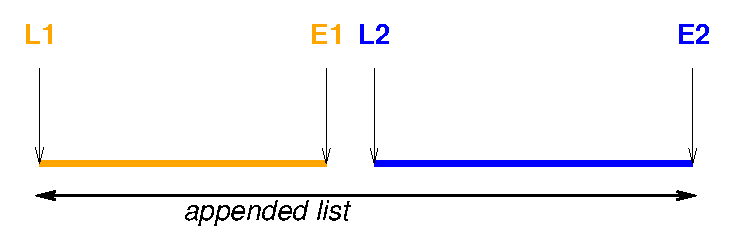
\includegraphics{appenddiff.ps}
%\caption{Appending difference lists}
%\end{figure}
%The situation is as shown in the figure. By setting E1 to L2, the second 
%list is appended to the end of the first list, and \verb'L1',\verb'E2' now
%represents the combined list. With this difference list representation,
%no traversal of the first list is needed, and the operation is done in
%constant time. It can thus be much more efficient, especially if the first
%list is long.

\section{More control structures}
    \subsection{Disjunction}
\index{disjunction} \index{;/2}
Disjunction is normally specified in Prolog by different clauses of
a predicate, but it can also be specified within a single clause by
the use of \verb';/2'. For example,

\begin{code}
atomic_particle(X) :- (X = proton ; X = neutron ; X = electron).
\end{code}

This is logically equivalent to: 

\begin{code}
atomic_particle(proton).
atomic_particle(neutron).
atomic_particle(electron).
\end{code}

    \subsection{Conditional}

\index{conditional} \index{->/2}
Conditionals can be specified using the \verb'->/2' operator.
In combination with \verb';/2', a conditional similar to `if-then-else' 
constructs of conventional language can be constructed:
\verb'X->Y;Z', where \verb'X', \verb'Y' and \verb'Z' can be one or more
goals,  means that if \verb'X' is true, then \verb'Y' will be
executed, otherwise \verb'Z'. Only the first solution of \verb'X' is
explored, so that on backtracking, no new solutions for \verb'X' will be
tried. In addition, if \verb'X' succeeds, then the `else' part, \verb'Z'
will never be tried. If \verb'X' fails, then the `then' part, \verb'Y',
will never be tried. An example of `if-then-else' is:
\begin{code}
max(X,Y, Max) :- 
   number(X), number(Y),
   (X > Y -> Max = X ; Max = Y).
\end{code}
where \verb'Max' is the bigger of the numbers \verb'X' or \verb'Y'.
Note the use of the brackets to make the scope of the if-then-else
clear and correct.


    \subsection{Call} 
\index{call}
\index{metacall}
One feature of Prolog is the equivalence of  programs and data -- both are
represented as terms. The predicate \verb'call' allows 
program terms (i.e. data) to be treated as goals: \verb'call(X)' will cause
\verb'X' to be treated as a goal and executed. Although at the time when 
the predicate is executed, \verb'X' has to be instantiated, it does not 
need to be instantiated (or even known) at compile time. For example, it
would in principle be
possible to define disjunction (\verb';') as follows:

\begin{code}
X ; Y :- call(X).
X ; Y :- call(Y).
\end{code}

%In addition, a Prolog program can construct a term at run-time, which is then 
%called as a goal.  This is sometimes used to ensure goals are compiled
%after earlier goals have already been executed, for
%example\footnote{The 'foreach' construct is described in the next chapter.}:
%\begin{verbatim}
%Y=A, call(foreach(A,[a,b,c]) do writeln(Y)).
%\end{verbatim}
%As required, this means the same as
%\begin{verbatim}
%foreach(A,[a,b,c]) do writeln(A).
%\end{verbatim}


\subsection{All Solutions}
\label{all-solutions}

In the pure computational model of Prolog, alternative solutions are
computed one-by-one on backtracking. Only one solution is available
at any time, while previous solutions disappear on backtracking:
\begin{quote}\begin{verbatim}
?- weekday(X).
X = mo
More
X = tu
More
X = we
More
...
\end{verbatim}\end{quote}
Sometimes it is useful to have all solution together in a list.
This can be achieved by using one of the all-solutions predicates
\index{findall/3}\index{setof/3}\index{bagof/3}findall/3, setof/3 or bagof/3:
\begin{quote}\begin{verbatim}
?- findall(X, weekday(X), List).
X = X
List = [mo, tu, we, th, fr, sa, su]
Yes
\end{verbatim}\end{quote}
\See{For the differences between findall/3, setof/3 and bagof/3
see the \eclipse{} Reference Manual.}


\section{Using Cut}
\label{cut}
\index{cut}
Cut (written as \verb'!') prunes away part of the Prolog search-space. This
can be a very powerful mechanism for improving the performance of programs,
and even the suppression of unwanted solutions. However, it can also be
easily misused and over-used. 

Cut does two things:

\begin{description}
\item[commit] Disregard any later clauses for the predicate.
\item[prune] Throw away all alternative solutions to the goals to the left of
 the cut.
\end{description}

\subsection{Commit to current clause}
\index{commit}

Consider the following encoding of the ``minimum'' predicate:
\begin{code}
min(X,Y, Min) :- X <Y, Min = X.
min(X,Y, Min) :- Y=<X, Min = Y.
\end{code}
Whilst logically correct, the behaviour of this encoding is
non-optimal for two reasons.  Consider the goal {\tt :- min(2,3,M)}.
Although the first clause succeeds, correctly instantiating $M$ to
$2$, Prolog leaves an open choice point.  If these clauses and goal
occur as part of a larger program and goal, a failure might occur
later, causing backtracking to this open choice point. 
Prolog would then, in vain, try to find another minimum using the
second clause for {\tt min}.  So there is a double drawback:
firstly, an open choice point consumes memory, and secondly the
unsuccessful evaluation of the second clause costs execution time.

To achieve the same logic, but more efficient behaviour, the
programmer can introduce a {\it cut}.
For example {\tt min} is typically encoded as follows:
\begin{code}
min(X,Y, Min) :- X<Y, !, Min = X.
min(X,Y, Y).
\end{code}
The cut removes the unnecessary choice point, which means that the
second clause will never be executed if the first clause passed the
cut.  This effectively makes the test in the second clause redundant,
and it can therefore be removed.

  \subsection{Prune alternative solutions}
\index{prune}
A cut may occur anywhere where a goal may occur, consider the following:
\begin{code}
first_prime(X, P) :-
    prime(X,P), !.
\end{code}
where \verb'first_prime' returns the first prime number smaller than \verb'X'.
In this case, it calls a predicate \verb'prime/2', which generates prime
numbers smaller than \verb'X', starting from the largest one. The effect of
the cut here is to prune away all the remaining solutions to \verb'prime(X,P)'
once the first one is generated, so that on backtracking, \verb'prime(X,P)'
is not tried for alternative solutions. The cut will also commit the execution
to this clause for \verb'first_prime/2', but as there is only one clause,
this has no visible effect.


%%----------------------------------------------------------------------
%\section{Prolog vs Imperative Languages}
%%----------------------------------------------------------------------
%\quickref{Comparison Prolog vs Imperative Programming}{
%\begin{tabular}{p{7cm}p{7cm}}
%{\bf Prolog} & {\bf Imperative Language} \\
%\hline
%\hline
%set of clauses & program \\
%\hline
%predicate (set of clauses with same name and arity) & procedure \\
%\hline
%clause (rule or fact) & if statement / one arm of nondeterministic case
%        statement / sequence of procedure calls \\
%\hline
%goal invocation & procedure call \\
%\hline
%unification & parameter passing / assignment / dynamic memory allocation /
%        conditional branching \\
%\hline
%backtracking & continuation passing / exception handling /
%        execution state manipulation \\
%\hline
%logical variable & pointer manipulation \\
%\hline
%tail recursion & iteration \\
%\end{tabular}
%}

%----------------------------------------------------------------------
\section{Common Pitfalls}
%----------------------------------------------------------------------
Prolog is different from conventional programming languages, and a common
problem is to program Prolog like a conventional language. Here are some
points to note:

\begin{itemize}
\item Unification is more powerful than normal case discrimination (see 
  section~\ref{unif}); 
\item Prolog procedure calls are more powerful than conventional procedure
calls. In particular, backtracking is possible (see section~\ref{back});
\end{itemize}

    \subsection{Unification works both ways}
\label{unif}
One common problem is to write a predicate expecting certain instantiation
patterns for the arguments, and then get unexpected results when the 
arguments do not conform to the expected pattern. An example is the
member relation, intended to check if an item \verb'Item' is a member of
a list or not. This might be written as:


\begin{code}
member(Item, [Item|_]).
member(Item, [_|List]) :- member(Item, List).
\end{code}

The expected usage assumes both \verb'Item' and the list are ground. In 
such cases, the above predicate does indeed check if \verb'Item' occurs in
the list given as a second argument. However, if either of the arguments are
not ground, then potentially unexpected behaviour might occur. Consider
the case where \verb'Item' is a variable, then the above predicate will 
enumerate the elements of the list successively through backtracking. On
the other hand, if any of the list elements of the list is a variable, they
would be unified with \verb'Item'. Other instantiation patterns for either
arguments can produce even more complex results. 

If the intended meaning is simply to check if \verb'Item' is a member of 
a list, this can be done by:

\begin{code}
  \% is_member(+Element, +List)
  \% check if Element is an element that occurs in a List of
  \% ground elements
is_member(Item, [Element|_]) :- Item == Element.
is_member(Item, [_|List]) :- nonvar(List), is_member(Item, List).
\end{code}

Note the use of comments to make clear the intention of the use of the
predicate. The convention used is that `+' indicates that an argument should
be instantiated (i.e. not a variable), `-' for an argument that should be
an uninstantiated variable, and '?' indicates that there is no restrictions
on the mode of the argument.

    \subsection{Unexpected backtracking}
\label{back}
Remember that when coding in Prolog, any predicate {\it may\/} be backtracked 
into. So correctness in Prolog requires:

\begin{itemize}
\item Predicate returns the correct answer when first called.
\item Predicate behaves correctly when backtracked into.
\end{itemize}

Recall that backtracking causes alternative choices to be explored, if
there are any.  Typically another choice corresponds to another clause
in the poredicate definition, but alternative choices may come from
disjunction (see above) or built-in predicates with multiple
(alternative) solutions. 
The programmer should make sure that a predicate will only produce
those solutions that are wanted. Excess alternatives can be removed by
coding the program not to produce them, or by the cut, or the conditional.

For example, to return only the {\it first\/} member, in the
\verb'is_member/2' example, 
the predicate can be coded using the cut, as follows:

\begin{code}
is_member(Item, [Element|_]) :- Item == Element, !.
is_member(Item, [_|List]) :- nonvar(List), is_member(Item, List).
\end{code}

\subsubsection{Using conditional}

Another way to remove excess choice points is the conditional:

\begin{code}
is_member(Item, [Element|List]) :- 
    ( Item == Element ->
        true 
    ;
        nonvar(List), is_member(Item, List)
    ).
\end{code}


\section{Exercises}

\begin{enumerate}

\item

Consider again the ``family tree'' example (see Section~\ref{syntax}).
As well as the \texttt{parent/2} predicate, suppose we have a
\texttt{male/1} predicate as follows:

\begin{code}
male(abe).
male(homer).
male(herbert).
male(bart).
\end{code}

Define a \texttt{brother/2} predicate, expressed just in terms of
\texttt{parent/2} and \texttt{male/1}.  Make sure Homer is not considered
his own brother.


\item

Consider the following alternative definition of \texttt{ancestor/2}:

\begin{code}
ancestor(X, Y) :- parent(X, Y).
ancestor(X, Y) :- ancestor(X, Z), parent(Z, Y).
\end{code}

What is wrong with this code?  What happens if you use it to find out
who Bart is an ancestor of?

\end{enumerate}

%HEVEA\cutend
